% =============================================================
% บทที่ 3 - วิธีการดำเนินงาน
% =============================================================

บทนี้นำเสนอกระบวนการและวิธีดำเนินการวิจัยสำหรับโครงงาน Pacegasus ซึ่งแบ่งออกเป็น 5 ขั้นตอนหลัก ได้แก่ (1) การศึกษาทฤษฎีและงานวิจัยที่เกี่ยวข้อง (2) การเก็บและวิเคราะห์ความต้องการ (3) การออกแบบและพัฒนาแอปพลิเคชันต้นแบบ (4) การทดสอบและปรับปรุงระบบ และ (5) การประเมินผล รวมถึงเครื่องมือที่ใช้ในการดำเนินงาน

\section{ขั้นตอนการดำเนินงาน}

\subsection{การศึกษาทฤษฎีและงานวิจัยที่เกี่ยวข้อง}

ขั้นตอนแรกของการวิจัยเริ่มต้นด้วยการทบทวนวรรณกรรมอย่างเป็นระบบ เพื่อสร้างฐานความรู้ที่แข็งแกร่งสำหรับการออกแบบระบบ กระบวนการดำเนินการมีดังนี้

\subsubsection{การรวบรวมเอกสารและงานวิจัย}

คณะผู้วิจัยทำการรวบรวมเอกสารและงานวิจัยที่เกี่ยวข้องจากฐานข้อมูลวิชาการชั้นนำ ได้แก่ PubMed, Google Scholar, IEEE Xplore และ ACM Digital Library โดยกำหนดคำค้นหาหลัก เช่น \textit{running application}, \textit{gamification physical activity}, \textit{self-determination theory exercise}, \textit{adaptive training machine learning}, \textit{session-RPE} และ \textit{ACWR injury prevention} กำหนดเกณฑ์การคัดเลือกงานวิจัยที่ตีพิมพ์ตั้งแต่ปี ค.ศ. 2018 เป็นต้นมา และงานวิจัยพื้นฐานที่สำคัญในช่วงก่อนหน้า

\subsubsection{การวิเคราะห์และสังเคราะห์กรอบแนวคิด}

หลังจากรวบรวมเอกสารแล้ว คณะผู้จัดทำวิเคราะห์จุดแข็งของกรอบทฤษฎีและกำหนดวิธีประยุกต์ใช้กับระบบ โดยใช้ทฤษฎีการกำหนดใจตนเอง (Self-Determination Theory:SDT) เป็นกรอบแนวคิดด้านแรงจูงใจ ใช้เทคนิคการเปลี่ยนพฤติกรรม (Behavior Change Techniques: BCTs) สำหรับเลือกกลไกที่มีหลักฐานสนับสนุน ใช้แนวคิด Gamification เพื่อสร้างการมีส่วนร่วมและการใช้งานต่อเนื่อง และใช้คุณลักษณะทางสังคมเพื่อเพิ่มความรู้สึกเชื่อมโยงระหว่างผู้ใช้งาน ผลลัพธ์ของขั้นตอนนี้คือกรอบแนวคิดที่เชื่อมโยงทฤษฎีกับการออกแบบ

\subsection{การเก็บและวิเคราะห์ความต้องการ}

\subsubsection{กลุ่มเป้าหมายและเกณฑ์การแบ่งระดับ}

กลุ่มเป้าหมายหลักของระบบคือผู้วิ่งระดับเริ่มต้นและระดับกลางที่มีสมาร์ตโฟนและต้องการพัฒนาพฤติกรรมการออกกำลังกายอย่างสม่ำเสมอ เกณฑ์การแบ่งระดับใช้ 4 มิติร่วมกันแทนการดูแค่ผลแข่งขัน: ระยะเวลาฝึกต่อเนื่อง, ปริมาณวิ่ง/สัปดาห์, ความถี่การซ้อม, ผลงานการแข่งขัน (ถ้ามี) ดังตารางที่ \ref{tab:runner-level}

\begin{table}[H]
\centering
\caption{เกณฑ์การแบ่งระดับนักวิ่งในระบบ Pacegasus}
\label{tab:runner-level}
\small
\begin{tabular}{|p{1.65cm}|p{1.85cm}|p{1.45cm}|p{1.35cm}|p{3.1cm}|}
\hline
\textbf{ระดับ} & \textbf{ฝึกต่อเนื่อง} & \textbf{วิ่ง/สัปดาห์} & \textbf{วันที่วิ่ง/สัปดาห์} & \textbf{ลักษณะการซ้อม} \\ \hline
Beginner & 0--8 เดือน / เพิ่งกลับมาวิ่ง & 8--25 กม. & 3--4 วัน & ยังไม่มี Speed Work เป็นระบบ; ยังไม่เคยแข่ง หรือ 5K แรก \\ \hline
Lower Intermediate & 1--2 ปีขึ้นไป & 25--50 กม. & 4--5 วัน & เริ่มมี Tempo/Interval 1--2 ครั้ง/สัปดาห์; จบ 10K--HM มาแล้วหลายครั้ง \\ \hline
Upper Intermediate & 2--4 ปีขึ้นไป & 50--100 กม. & 4--5 วัน & มี Tempo/Interval 1--2 ครั้ง/สัปดาห์; จบ 21K--HM มาแล้วหลายครั้ง และตั้งเป้า PB \\ \hline

\end{tabular}
\end{table}

\subsubsection{วิธีการสุ่มตัวอย่างและขนาดตัวอย่าง}

การศึกษานี้ใช้การสุ่มตัวอย่างแบบเจาะจง ณ สถานที่ร่วมกับการสุ่มแบบมีระบบ (on-site systematic intercept sampling) โดยเก็บข้อมูล ณ สถานที่ออกกำลังกาย 3 แห่งในจังหวัดขอนแก่น ได้แก่ สวนเกษตร มหาวิทยาลัยขอนแก่น สนามกีฬา 50 ปี มหาวิทยาลัยขอนแก่น และบึงศรีฐาน (ดูรายละเอียดสถานที่ในหัวข้อ~\ref{sec:research-sites})
% TODO: ระบุค่า n ของการสุ่มแบบมีระบบให้ชัดเจน เช่น "ทุกคนที่ 3" หรือ "ทุกคนที่ 5" ที่ผ่านจุดสำรวจ
โดยกำหนดให้เข้าหาผู้เข้าร่วมทุกคนที่ [n] คนที่ผ่านจุดสำรวจ ในช่วงเวลาที่ครอบคลุมทั้งช่วงเช้าและเย็น รวมถึงวันธรรมดาและวันหยุด เพื่อลดความเอนเอียงจากการเลือกกลุ่มตัวอย่างของผู้สำรวจเอง (interviewer selection bias) และลดผลกระทบจากลักษณะกลุ่มผู้ออกกำลังกายที่แตกต่างกันในแต่ละช่วงเวลา

จากกลุ่มที่ถูกเข้าหาตามระบบสุ่มดังกล่าว ผู้สำรวจจะคัดกรองเพิ่มเติมด้วยเกณฑ์เชิงพฤติกรรม (purposive/criterion-based screening) โดยพิจารณาเฉพาะผู้ที่พกโทรศัพท์สมาร์ตโฟนหรือสวมใส่นาฬิกาวิ่ง (running/GPS watch) ขณะออกกำลังกาย เพื่อให้กลุ่มตัวอย่างสะท้อนลักษณะผู้ใช้เป้าหมายของระบบ \textit{Pacegasus} ได้ตรงยิ่งขึ้น วิธีการสุ่มโดยรวมจึงจัดเป็น systematic intercept sampling ร่วมกับ purposive screening ซึ่งยังคงเป็นการสุ่มแบบไม่อาศัยความน่าจะเป็น (non-probability sampling)

ผู้เข้าร่วมต้องมีอายุ 18 ปีขึ้นไป ออกกำลังกายหรือวิ่งอย่างน้อยสัปดาห์ละ 1 ครั้งในช่วง 3 เดือนที่ผ่านมา และพกโทรศัพท์สมาร์ตโฟนหรือสวมใส่นาฬิกาวิ่งขณะออกกำลังกาย เกณฑ์การออกกำลังกายอย่างน้อยสัปดาห์ละ 1 ครั้งใช้เพื่อจำแนกผู้ออกกำลังกายสม่ำเสมอ (regular exerciser) ออกจากผู้ที่ไม่ได้ออกกำลังกายเป็นประจำ \cite{childs2014} ส่วนกรอบเวลาย้อนหลัง 3 เดือนใช้เพื่อลดผลกระทบจากความผันผวนระยะสั้นของพฤติกรรม (เช่น สภาพอากาศ ช่วงสอบ หรือการเจ็บป่วยชั่วคราว) และสะท้อนพฤติกรรมเชิงนิสัยที่คงที่มากกว่าการถามเฉพาะสัปดาห์ล่าสุด

เนื่องจากไม่มีบัญชีรายชื่อประชากรนักวิ่งทั้งหมด (sampling frame) จึงกำหนดขนาดตัวอย่างโดยอ้างอิงสูตร Cochran สำหรับการประมาณสัดส่วน \cite{cochran1977} ดังนี้

\begin{center}
    $n_0 = \dfrac{Z^2p(1-p)}{d^2}$
\end{center}

และปรับขนาดตัวอย่างสำหรับประชากรจำกัดด้วยสูตร

\begin{center}
    $n = \dfrac{n_0}{1+\dfrac{n_0-1}{N}}$
\end{center}

โดย $n_0$ คือขนาดตัวอย่างเริ่มต้น $n$ คือขนาดตัวอย่างหลังปรับตามจำนวนประชากร $N$ คือจำนวนประชากรโดยประมาณ $Z$ คือค่ามาตรฐานตามระดับความเชื่อมั่น $p$ คือสัดส่วนที่คาดการณ์ และ $d$ คือค่าความคลาดเคลื่อน

การศึกษานี้กำหนดระดับความเชื่อมั่นร้อยละ 95 ($Z=1.96$) กำหนด $p=0.50$ เนื่องจากยังไม่มีข้อมูลสัดส่วนของคุณลักษณะที่ศึกษาล่วงหน้า ค่านี้ให้ค่าความแปรปรวนสูงสุด (most conservative estimate) จึงเหมาะสมที่สุดในกรณีที่ไม่มีข้อมูลนำร่อง เนื่องจากโครงงานนี้อยู่ในลักษณะการประเมินต้นแบบระบบ (prototype/formative evaluation) เพื่อสำรวจความต้องการและทดสอบการใช้งานเบื้องต้น มากกว่าการอนุมานเชิงสถิติในวงกว้าง จึงกำหนดค่าความคลาดเคลื่อน $d=0.25$ ซึ่งสอดคล้องกับแนวทางการทดสอบการใช้งาน (usability testing) ที่ระบุว่ากลุ่มตัวอย่างขนาดเล็ก (ประมาณ 5--15 คน) เพียงพอต่อการค้นพบปัญหาการใช้งานส่วนใหญ่ของระบบ โดยอ้างอิงแบบจำลองของ Nielsen และ Landauer \cite{nielsen1993} ที่แสดงว่าผู้ใช้ทดสอบ 5 คนสามารถค้นพบปัญหาการใช้งานได้ประมาณร้อยละ 85

เนื่องจากวิธีสุ่มตัวอย่างที่ใช้เป็นแบบไม่อาศัยความน่าจะเป็น ขนาดตัวอย่างที่คำนวณได้จากสูตร Cochran ในที่นี้จึงใช้เป็นเกณฑ์อ้างอิงขั้นต่ำ (minimum reference threshold) เพื่อประกอบการวางแผนเก็บข้อมูล มิได้ใช้เพื่ออ้าง representativeness ทางสถิติต่อประชากรทั้งหมด จากค่าดังกล่าวจะได้ขนาดตัวอย่างเริ่มต้น $n_0=15.37$ คน เมื่อนำไปปรับตามประชากรเป้าหมายประมาณ 50--100 คน
% TODO: ระบุที่มาของ N ≈ 50--100 คน เช่น จำนวนสมาชิกกลุ่ม Facebook/Strava ที่เกี่ยวข้อง หรือจำนวนที่สังเกตได้จากการสำรวจเบื้องต้น (pilot observation) ที่ทั้ง 3 สถานที่
จะได้ขนาดกลุ่มตัวอย่างขั้นต่ำประมาณ 12--14 คน จึงกำหนดเป้าหมายผู้ตอบแบบสอบถามที่สมบูรณ์จำนวน 15 คน โดยจัดสรรแบบแบ่งชั้น (stratified allocation) ตามระดับผู้วิ่งในตารางที่~\ref{tab:runner-level} คือ Beginner, Lower Intermediate และ Upper Intermediate ระดับละ 5 คน เพื่อให้แต่ละระดับประสบการณ์มีตัวแทนเพียงพอสำหรับการค้นพบปัญหาการใช้งานตามแนวทางของ Nielsen และ Landauer \cite{nielsen1993}

ข้อจำกัดของวิธีการสุ่มตัวอย่าง กลุ่มตัวอย่างจำกัดเฉพาะผู้ที่ออกกำลังกาย ณ 3 สถานที่ในจังหวัดขอนแก่นและมีอุปกรณ์ติดตามการวิ่งอยู่แล้ว ผลการศึกษาจึงสะท้อนพฤติกรรมของผู้ใช้เทคโนโลยีติดตามการวิ่งในบริบทพื้นที่ศึกษาเป็นหลัก ไม่ครอบคลุมนักวิ่งในพื้นที่อื่น ผู้ออกกำลังกายในสถานที่ปิด (ฟิตเนส, สนามในบ้าน) หรือผู้ที่ไม่ใช้อุปกรณ์ติดตามใด ๆ ซึ่งอาจเป็นกลุ่มที่มีศักยภาพเป็นผู้ใช้ใหม่ของระบบในอนาคตแต่ไม่ถูกรวมในการศึกษานี้

คัดเลือกผู้สมัครใจแบบเจาะจงจำนวน 2--4 คน โดยพิจารณาผู้ที่มีประสบการณ์วิ่งหรือออกกำลังกายอย่างสม่ำเสมอ เพื่อรับฟังปัญหา ความต้องการ และข้อเสนอแนะเชิงลึกประกอบการออกแบบระบบ การสัมภาษณ์ในส่วนนี้มุ่งเก็บข้อมูลสนับสนุนการออกแบบต้นแบบ มิได้มุ่งอ้างอิงความอิ่มตัวของข้อมูลเชิงคุณภาพ

\subsubsection{เครื่องมือและวิธีการเก็บข้อมูล}

เครื่องมือที่ใช้ประกอบด้วยแบบสอบถามออนไลน์ผ่าน Google Forms และแนวคำถามสัมภาษณ์เชิงลึกแบบกึ่งโครงสร้าง แบบสอบถามครอบคลุมพฤติกรรมการวิ่งในปัจจุบัน ปัญหาและอุปสรรค คุณลักษณะที่ต้องการในแอปพลิเคชัน และความคุ้นเคยกับ Gamification ส่วนการสัมภาษณ์ใช้เพื่อทำความเข้าใจแรงจูงใจและพฤติกรรมของผู้ใช้งานในระดับลึก

\subsubsection{วิธีการวิเคราะห์ข้อมูล}

ข้อมูลเชิงปริมาณจากแบบสอบถามวิเคราะห์ด้วยค่าเฉลี่ย ส่วนเบี่ยงเบนมาตรฐาน และการแจกแจงความถี่ ส่วนข้อมูลเชิงคุณภาพจากการสัมภาษณ์วิเคราะห์เชิงธีม (Thematic Analysis) เพื่อระบุรูปแบบและประเด็นที่ปรากฏซ้ำ ผลการวิเคราะห์นำไปกำหนดความต้องการของระบบ ครอบคลุมฟีเจอร์ด้าน Social Features, Gamification Elements และการเชื่อมต่อข้อมูลกิจกรรมจาก Strava API ผ่าน OAuth 2.0

\subsection{การออกแบบและพัฒนาแอปพลิเคชันต้นแบบ}

ขั้นตอนที่สามเป็นหัวใจหลักของโครงงาน ซึ่งครอบคลุมทั้งกระบวนการออกแบบ UX/UI และการพัฒนาระบบในเชิงเทคนิค

\subsubsection{การออกแบบประสบการณ์และส่วนติดต่อผู้ใช้(UX/UI Design)}

การออกแบบ UX/UI ดำเนินการโดยใช้ Figma เป็นเครื่องมือหลักในการสร้าง Wireframe และ Hi-fi Prototype กระบวนการออกแบบเริ่มต้นจากการสร้าง User Persona จากผลการวิเคราะห์ความต้องการ จากนั้นจัดทำ User Flow สำหรับเส้นทางสำคัญของผู้ใช้ เช่น กระบวนการลงทะเบียน การตั้งค่าแผนการฝึก การบันทึกกิจกรรม และการมีปฏิสัมพันธ์ทางสังคม ต่อมาจัดทำ Wireframe ระดับ Low-fidelity เพื่อทดสอบการจัดวางองค์ประกอบ และสุดท้ายพัฒนาเป็น Hi-fidelity Prototype ที่แสดงรายละเอียดด้านสี ตัวอักษร และองค์ประกอบภาพ

\subsubsection{สถาปัตยกรรมระบบ}

ระบบ Pacegasus ออกแบบโดยใช้สถาปัตยกรรมแบบ Client--Server แบ่งออกเป็น 3 ชั้นหลัก ดังนี้

ชั้นที่ 1 คือฝั่งแอปพลิเคชัน (Client Side) พัฒนาด้วย Flutter ซึ่งเป็น Cross-platform Framework ที่รองรับ Android และ iOS จากโค้ดชุดเดียว โดยใช้ภาษา Dart ภายในแอปพลิเคชันแบ่งเป็น 4 โมดูล ได้แก่ Activity Tracking Module ที่ใช้ GPS และ Accelerometer, Gamification Module สำหรับจัดการคะแนน เหรียญตรา เลเวล และ Story Mode, Social Module สำหรับระบบเพื่อน กลุ่ม และกิจกรรมร่วม และ AI Coach Module สำหรับแสดงผลและรับส่งข้อมูลกับ Backend

ชั้นที่ 2 คือฝั่งเซิร์ฟเวอร์ (Backend/Server Side) พัฒนาด้วย Express.js บน Node.js ซึ่งรองรับการทำงานแบบ Asynchronous และ Real-time โดยมี REST API สำหรับจัดการข้อมูลผู้ใช้และกิจกรรม WebSocket ผ่าน Socket.io สำหรับการแจ้งเตือนและการอัปเดตกระดานผู้นำ และ Adaptive Training Engine สำหรับปรับแผนฝึก

ชั้นที่ 3 คือฐานข้อมูล (Database Layer) ใช้ PostgreSQL เป็นระบบจัดการฐานข้อมูลหลัก การออกแบบ Database Schema ครอบคลุมตาราง Users, Activities, TrainingPlans, WellnessCheckins, Badges, Clubs และ LeaderboardEntries

การสื่อสารระหว่าง Client และ Backend ทำผ่าน Request/Response แบบมาตรฐาน โดย Backend ทำหน้าที่เชื่อมต่อและประมวลผลข้อมูลกับฐานข้อมูลและบริการภายนอกทั้งหมด ดังภาพที่~\ref{fig:system-architecture}

\begin{figure}[H]
\centering
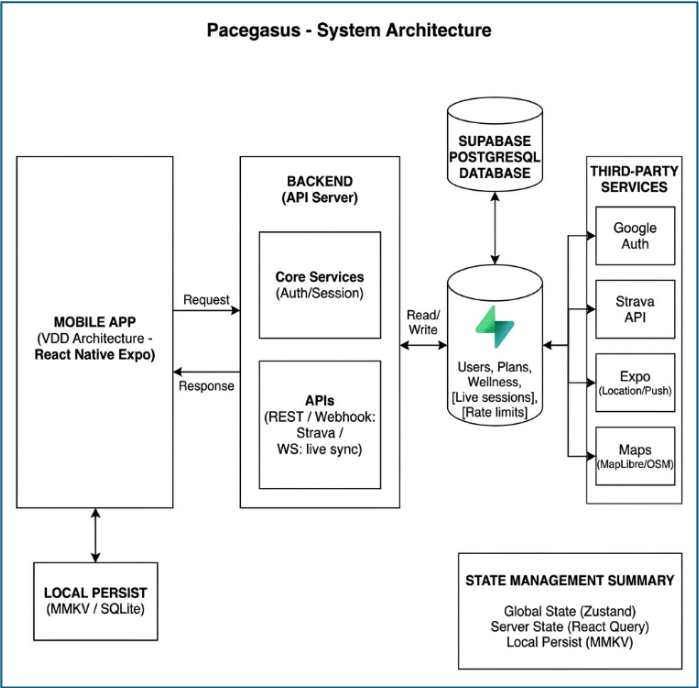
\includegraphics[width=0.95\textwidth]{images/Chapter3_system.png}
\caption{สถาปัตยกรรมระบบ (System Architecture)}
\label{fig:system-architecture}
\end{figure}

\subsubsection{การพัฒนา Adaptive Training Engine}

Adaptive Training Engine เป็นองค์ประกอบที่มีความซับซ้อนสูงสุดในระบบ ประกอบด้วย 3 ส่วนหลัก 

ส่วนที่ 1 คือ Daily Wellness Check-in รับข้อมูลจากผู้ใช้ทุกเช้าในรูปแบบระดับ 1--5 ได้แก่ ระดับความเหนื่อยล้าสะสม คุณภาพการนอนหลับ ความเจ็บปวดของกล้ามเนื้อ ระดับความเครียด และระดับแรงจูงใจในวันนั้น

ส่วนที่ 2 คือโมดูลคำนวณ Session-RPE และ ACWR หลังจบการวิ่ง ระบบเก็บข้อมูล sRPE (ระยะเวลา $\times$ RPE) เพื่อนำไปประเมินความเสี่ยงต่อการบาดเจ็บ

ส่วนที่ 3 คือโมดูล Machine Learning ใช้อัลกอริทึม Decision Tree หรือ Random Forest โดยรับข้อมูล Wellness Check-in ค่า ACWR ประวัติการฝึก 4 สัปดาห์ และแผนเป้าหมายของผู้ใช้ เพื่อให้คำแนะนำสำหรับวันถัดไป เช่น ฝึกตามแผน ลดความหนัก หรือพักผ่อน

\subsubsection{ระดับต้นแบบที่พัฒนา}

ต้นแบบแอปพลิเคชันที่พัฒนาในระยะนี้รองรับฟีเจอร์หลัก ได้แก่ การติดตามกิจกรรมด้วย GPS ระบบ Gamification พื้นฐาน เช่น คะแนน เหรียญตรา เลเวล และภารกิจรายสัปดาห์ ระบบ Social Interaction เบื้องต้น ได้แก่ การเพิ่มเพื่อน กระดานผู้นำ และการให้กำลังใจ และ Adaptive Training Engine เวอร์ชันทดลองที่ใช้ Wellness Check-in และ sRPE ในการปรับแผน

\subsection{การทดสอบและปรับปรุงระบบ}

ขั้นตอนที่สี่มุ่งตรวจสอบความถูกต้องและความสามารถในการใช้งานของระบบก่อนการประเมินผลอย่างเป็นทางการ

\subsubsection{การทดสอบระบบในเชิงเทคนิค}

การทดสอบระบบในเชิงเทคนิคแบ่งเป็น 2 ระดับ ได้แก่ Unit Testing ซึ่งทดสอบความถูกต้องของฟังก์ชันในแต่ละโมดูล โดยใช้ Jest/Mocha สำหรับ Backend และ flutter test สำหรับ Frontend และ Integration Testing ซึ่งทดสอบการทำงานร่วมกันระหว่างโมดูล เช่น การส่งข้อมูลจาก Activity Tracking Module ไปยัง Adaptive Training Engine และการอัปเดต Leaderboard แบบ Real-time

\subsubsection{การทดสอบแบบ Beta Test}

การทดสอบ Beta Test ดำเนินการกับผู้ใช้จริงที่คัดเลือกจากกลุ่มผู้ตอบแบบสอบถามที่ผ่านเกณฑ์และแสดงความสมัครใจเข้าร่วมทดสอบต่อ จำนวน 2--5 คน ใช้สมาร์ตโฟนเป็นประจำ มีประสบการณ์วิ่งต่อเนื่องไม่น้อยกว่า 1 เดือน และยินยอมให้เก็บข้อมูลการใช้งานเป็นระยะเวลา 2--4 สัปดาห์ ข้อมูลที่เก็บประกอบด้วย Log Data และ App Analytics เช่น จำนวนครั้งใช้งาน ระยะทาง และอัตราการเปิดแอปพลิเคชัน แบบสอบถามความพึงพอใจรายสัปดาห์ และการสัมภาษณ์ข้อเสนอแนะหลังใช้งาน เนื่องจากข้อจำกัดด้านเวลาและทรัพยากรของโครงงานระดับสัมมนา ขนาดกลุ่มนี้จึงต่ำกว่าเกณฑ์ที่แนะนำสำหรับการทดสอบสถิติอย่างเป็นทางการ (เช่น 12 คน/กลุ่มตามข้อเสนอของ Julious \cite{julious2005}) ผลจากการทดสอบนี้จึงใช้เป็นข้อมูลเชิงสำรวจ (exploratory) เพื่อประเมินต้นแบบระบบในระยะพัฒนา มิได้มุ่งอ้างอิงเชิงสถิติต่อประชากรผู้ใช้ในวงกว้าง

\clearpage
\subsection{การประเมินผล}

\subsubsection{ตัวชี้วัดเชิงปริมาณ (เกณฑ์อ้างอิงเชิงพรรณนา)}

กำหนดค่าเป้าหมายอ้างอิงเพื่อประเมินแนวโน้มการใช้งานในเชิงพรรณนา ได้แก่ (1) จำนวนครั้งใช้งานต่อสัปดาห์ (2) ร้อยละการเปลี่ยนแปลงของระยะทางรวมเมื่อเทียบกับช่วงก่อนใช้งาน และ (3) จำนวนผู้ที่ยังใช้งานต่อเนื่องภายใน 4 สัปดาห์ (retention) โดยรายงานผลเป็นรายบุคคล (case-level) ควบคู่กับค่าเฉลี่ยและช่วงค่าต่ำสุด-สูงสุดของกลุ่ม แทนการรายงานเป็นร้อยละรวมเทียบกับเกณฑ์ผ่าน/ไม่ผ่านเพียงอย่างเดียว เนื่องจากขนาดกลุ่มตัวอย่างที่เล็ก (2--5 คน) ทำให้ค่าร้อยละเชิงเดี่ยวไม่สะท้อนนัยสำคัญทางสถิติที่แท้จริง

\subsubsection{ตัวชี้วัดเชิงคุณภาพ}

ประกอบด้วยคะแนนความพึงพอใจโดยรวมของผู้เข้าร่วมแต่ละคน (รายงานเป็นรายบุคคลและค่าเฉลี่ย) และความรู้สึกสนุกกับระดับแรงจูงใจที่เปลี่ยนแปลงเมื่อเปรียบเทียบก่อนและหลังการใช้งาน ซึ่งเก็บผ่านแบบสอบถามรายสัปดาห์และการสัมภาษณ์

\subsubsection{ตัวชี้วัดสำหรับ Adaptive Training Engine}

เนื่องจากวัตถุประสงค์หนึ่งของโครงงานคือการพัฒนา Adaptive Training Engine เพื่อปรับแผนฝึกอัตโนมัติให้เหมาะสมกับผู้ใช้แต่ละคน จึงกำหนดตัวชี้วัดเพิ่มเติมโดยเฉพาะสำหรับส่วนนี้ นอกเหนือจากตัวชี้วัดการใช้งานแอปพลิเคชันโดยรวม ได้แก่ (1) อัตราการปฏิบัติตามคำแนะนำของระบบ (adherence rate) คือสัดส่วนวันที่ผู้ใช้ฝึกซ้อมสอดคล้องกับคำแนะนำที่ Engine เสนอในแต่ละวัน (ฝึกตามแผน ลดความหนัก หรือพักผ่อน) เทียบกับจำนวนวันทั้งหมดในช่วง Beta Test ซึ่งเป็นตัวชี้วัดที่ใช้ทั่วไปในการประเมินความสำเร็จของโปรแกรมติดตามและปรับแผนการฝึกในนักกีฬา \cite{mcguigan2023} และ (2) ความไว้วางใจและความรู้สึกว่าคำแนะนำมีความเหมาะสมกับตนเอง (perceived trust and appropriateness) ซึ่งเก็บผ่านแบบสอบถามรายสัปดาห์และการสัมภาษณ์ โดยอ้างอิงข้อค้นพบจากงานวิจัยระบบวางแผนฝึกวิ่งแบบปรับตัวได้รายวันด้วย AI ที่ระบุว่าความไว้วางใจของนักวิ่งต่อคำแนะนำเป็นปัจจัยสำคัญที่กำหนดว่าคำแนะนำจะถูกนำไปปฏิบัติจริงหรือไม่ \cite{nilsson2023} ทั้งนี้แนวทางการประเมินความพึงพอใจและผลของการปรับภาระการฝึกด้วยอัลกอริทึมยังสอดคล้องกับงานวิจัยที่แสดงว่าการปรับแผนฝึกแบบปรับตัวได้ (adaptive load control) ส่งผลให้ความพึงพอใจของผู้ใช้เพิ่มขึ้นและมีแนวโน้มลดอัตราการบาดเจ็บได้มากกว่าการวางแผนฝึกแบบตายตัว \cite{xia2025}

\subsubsection{วิธีการวิเคราะห์และการอภิปรายผล}

การวิเคราะห์ข้อมูลเชิงปริมาณใช้สถิติเชิงพรรณนา (descriptive statistics) เป็นหลัก ได้แก่ ค่าเฉลี่ย ค่ามัธยฐาน และช่วงค่าของการเปลี่ยนแปลงก่อน-หลังการใช้งานรายบุคคล เพื่อสังเกตแนวโน้มเบื้องต้นของพฤติกรรมการใช้งาน ส่วนการทดสอบ Paired t-test และ Wilcoxon Signed-rank Test คงไว้เป็นการวิเคราะห์เสริมเชิงสำรวจ (supplementary exploratory analysis) เท่านั้น โดยระบุข้อจำกัดด้านอำนาจการทดสอบทางสถิติ (statistical power) อันเนื่องมาจากขนาดกลุ่มตัวอย่างที่น้อย และไม่ใช้ผลดังกล่าวเป็นข้อสรุปเชิงนัยสำคัญทางสถิติ

ข้อมูลเชิงคุณภาพจากการสัมภาษณ์วิเคราะห์โดยการวิเคราะห์เชิงธีม (thematic analysis) เพื่อระบุรูปแบบและประเด็นสำคัญที่ปรากฏในประสบการณ์การใช้งานของผู้เข้าร่วมแต่ละคน การอภิปรายผลจะอ้างอิงทฤษฎี Self-Determination Theory (SDT) และ Behavior Change Techniques (BCTs) เพื่ออธิบายว่าการเปลี่ยนแปลงด้านแรงจูงใจที่สังเกตได้ในแต่ละกรณีเกิดจากฟีเจอร์ใดของระบบ โดยนำเสนอในลักษณะกรณีศึกษา (case-based synthesis) ที่เชื่อมโยงข้อมูลเชิงปริมาณและเชิงคุณภาพของผู้เข้าร่วมแต่ละคนเข้าด้วยกัน

\subsubsection{ข้อจำกัดของการประเมินผล}

เนื่องจากขนาดกลุ่มตัวอย่าง Beta Test ที่จำกัด (2--5 คน) ผลการประเมินจึงเหมาะสำหรับใช้เป็นหลักฐานเชิงสำรวจ (formative evidence) เพื่อปรับปรุงต้นแบบระบบในระยะพัฒนา มิใช่หลักฐานเชิงยืนยัน (confirmatory evidence) ที่สามารถอ้างอิงหรือขยายผลไปยังผู้ใช้กลุ่มใหญ่ได้ ผลการวิเคราะห์เชิงสถิติที่รายงานจึงควรตีความด้วยความระมัดระวัง และใช้ประกอบการตัดสินใจเชิงออกแบบร่วมกับข้อมูลเชิงคุณภาพเป็นสำคัญ

\subsubsection{สถานที่ดำเนินการวิจัย}
\label{sec:research-sites}

การวิจัยเก็บข้อมูลในพื้นที่หลัก 3 แห่งบริเวณมหาวิทยาลัยขอนแก่น ได้แก่ บึงศรีฐาน (ระยะทางต่อรอบประมาณ 1.5 กิโลเมตร) สวนเกษตร (ประมาณ 2.5 กิโลเมตร) และสนาม 50 ปีมหาวิทยาลัยขอนแก่น (ประมาณ 800 เมตร) ซึ่งเป็นพื้นที่ที่มีนักศึกษาและประชาชนมาออกกำลังกายเป็นประจำ

\subsection{สรุปขั้นตอนการวิจัย}

กระบวนการวิจัยทั้ง 5 ขั้นตอนมีความเชื่อมโยงกันอย่างเป็นระบบ โดยผลลัพธ์ของแต่ละขั้นตอนเป็น Input ของขั้นตอนถัดไป ขั้นตอนที่ 1 (ทบทวนวรรณกรรม) ให้กรอบแนวคิดสำหรับการออกแบบ ขั้นตอนที่ 2 (วิเคราะห์ความต้องการ) ให้ข้อกำหนดความต้องการของระบบ ขั้นตอนที่ 3 (ออกแบบและพัฒนา) ได้ต้นแบบแอปพลิเคชัน ขั้นตอนที่ 4 (ทดสอบและปรับปรุง) รับประกันคุณภาพของระบบก่อนการประเมิน และขั้นตอนที่ 5 (ประเมินผล) ให้ข้อมูลเชิงประจักษ์เพื่อยืนยันประสิทธิผลของระบบและนำไปสู่ข้อสรุปและข้อเสนอแนะในบทที่ 5

\begin{table}[H]
\centering
\caption{สรุปขั้นตอน เครื่องมือ และผลลัพธ์ของการวิจัย}
\label{tab:research-summary}
\small
\begin{tabular}{|p{1.8cm}|p{2.7cm}|p{2.5cm}|p{2.7cm}|}
\hline
\textbf{ขั้นตอน} & \textbf{กิจกรรมหลัก} & \textbf{เครื่องมือที่ใช้} & \textbf{ผลลัพธ์} \\ \hline
1. ทบทวนวรรณกรรม & รวบรวมและสังเคราะห์งานวิจัย & Google Scholar, PubMed, IEEE & Conceptual Framework \\ \hline
2. วิเคราะห์ความต้องการ & แบบสอบถามและสัมภาษณ์ & Google Forms, Semi-structured Interview & System Requirements \\ \hline
3. ออกแบบและพัฒนา & UX/UI Design และ Coding & Figma, Flutter, Express.js, PostgreSQL & Working Prototype \\ \hline
4. ทดสอบและปรับปรุง & Unit/Integration/Beta Test & Jest, Mocha, Flutter Test & Refined System \\ \hline
5. ประเมินผล & วัดตัวชี้วัดและวิเคราะห์ผล & Paired \textit{t}-test, Thematic Analysis & Research Findings \\ \hline
\end{tabular}
\end{table}

\section{เครื่องมือที่ใช้ในการดำเนินงาน}

\subsection{ฮาร์ดแวร์}

การพัฒนาและทดสอบระบบใช้คอมพิวเตอร์ส่วนบุคคลสำหรับออกแบบและพัฒนาแอปพลิเคชัน โดยมีรายละเอียดของฮาร์ดแวร์ที่ใช้แสดงดังตารางที่~\ref{tab:hardware-tools}

\begin{table}[H]
\centering
\caption{รายการฮาร์ดแวร์ที่ใช้ในการพัฒนา}
\label{tab:hardware-tools}
\small
\begin{tabular}{|c|p{4.1cm}|p{5.1cm}|}
\hline
\textbf{ลำดับ} & \textbf{รายการ} & \textbf{รายละเอียด} \\ \hline
1 & หน่วยประมวลผล & AMD Ryzen 7 8700F \\ \hline
2 & หน่วยความจำหลัก & RAM ขนาด 16 GB \\ \hline
3 & หน่วยจัดเก็บข้อมูล & SSD ขนาด 446 GB \\ \hline
4 & จอภาพ & ขนาด 23 นิ้ว \\ \hline
\end{tabular}
\end{table}

\subsection{ซอฟต์แวร์}

เครื่องมือซอฟต์แวร์ที่ใช้ในการดำเนินงานแสดงดังตารางที่~\ref{tab:software-tools} โดย Flutter เป็นเฟรมเวิร์กสำหรับพัฒนาแอปพลิเคชันและใช้ภาษา Dart ส่วน Express.js เป็นเฟรมเวิร์กสำหรับพัฒนาระบบฝั่งเซิร์ฟเวอร์ที่ทำงานบน Node.js และใช้ภาษา JavaScript

\begin{table}[H]
\centering
\caption{รายการซอฟต์แวร์ที่ใช้ในการพัฒนา}
\label{tab:software-tools}
\small
\begin{tabular}{|c|p{3.1cm}|p{2.2cm}|p{3.6cm}|}
\hline
\textbf{ลำดับ} & \textbf{ซอฟต์แวร์} & \textbf{เวอร์ชัน} & \textbf{วัตถุประสงค์} \\ \hline
1 & Windows 11 Home & 25H2 & ระบบปฏิบัติการสำหรับพัฒนาและทดสอบระบบ \\ \hline
2 & Dart & 3.13 & ภาษาที่ใช้พัฒนาแอปพลิเคชันด้วย Flutter \\ \hline
3 & Flutter & 3.47.0 & เฟรมเวิร์กสำหรับพัฒนาแอปพลิเคชัน \\ \hline
4 & Node.js & 24.18.1 LTS & สภาพแวดล้อมสำหรับรันระบบฝั่งเซิร์ฟเวอร์ \\ \hline
5 & Express.js & 5.2.1 & เฟรมเวิร์กสำหรับพัฒนา REST API ด้วยภาษา JavaScript \\ \hline
6 & PostgreSQL & 18.4 & ระบบจัดการฐานข้อมูล \\ \hline
7 & Visual Studio Code & 1.133 & โปรแกรมแก้ไขและพัฒนาซอร์สโค้ด \\ \hline
8 & Git for Windows & 2.53.0(3) & ระบบควบคุมเวอร์ชันของซอร์สโค้ด \\ \hline
\end{tabular}
\end{table}

\section{แผนการดำเนินงาน}

แผนการดำเนินงานของโครงงานกำหนดระยะเวลา 10 เดือน โดยลำดับกิจกรรมและช่วงเวลาดำเนินงานแสดงดังตารางที่~\ref{tab:gantt-chart}

\begin{table}[H]
\centering
\caption{แผนการดำเนินงาน (Gantt Chart)}
\label{tab:gantt-chart}
\scriptsize
\begin{tabular}{|c|p{3.6cm}|*{10}{c|}}
\hline
\textbf{ลำดับ} & \textbf{กิจกรรม} & \rotatebox{90}{\textbf{เดือน 1}} & \rotatebox{90}{\textbf{เดือน 2}} & \rotatebox{90}{\textbf{เดือน 3}} & \rotatebox{90}{\textbf{เดือน 4}} & \rotatebox{90}{\textbf{เดือน 5}} & \rotatebox{90}{\textbf{เดือน 6}} & \rotatebox{90}{\textbf{เดือน 7}} & \rotatebox{90}{\textbf{เดือน 8}} & \rotatebox{90}{\textbf{เดือน 9}} & \rotatebox{90}{\textbf{เดือน 10}} \\ \hline
1 & ศึกษาทฤษฎีและงานวิจัย & $\bullet$ & $\bullet$ &  &  &  &  &  &  &  &  \\ \hline
2 & การเก็บและวิเคราะห์ความต้องการ &  & $\bullet$ & $\bullet$ &  &  &  &  &  &  &  \\ \hline
3 & ทดสอบการเชื่อมต่อข้อมูล &  &  &  & $\bullet$ &  &  &  &  &  &  \\ \hline
4 & การออกแบบระบบและต้นแบบ &  &  &  & $\bullet$ & $\bullet$ & $\bullet$ &  &  &  &  \\ \hline
5 & พัฒนาแอปพลิเคชัน &  &  &  &  &  & $\bullet$ & $\bullet$ & $\bullet$ &  &  \\ \hline
6 & ทดสอบและปรับปรุง &  &  &  &  &  &  &  & $\bullet$ & $\bullet$ &  \\ \hline
7 & ประเมินผล &  &  &  &  &  &  &  &  & $\bullet$ & $\bullet$ \\ \hline
\end{tabular}
\end{table}